% Szglab4
% ===========================================================================
%
\chapter{Grafikus felület specifikációja}

\thispagestyle{fancy}

\section{A grafikus interfész}
%\comment{A menürendszer, a kezelői felület grafikus képe. A grafikus felület megjelenését, a használt ikonokat, stb screenshot-szerű képekkel kell bemutatni. Az építészetben ez a homlokzati terv.}
A szoftvert elindítva megjelenik egy grafikus ablak a következő tartalommal:

\begin{figure}[H]
\begin{center}
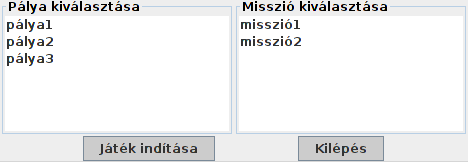
\includegraphics[width=10cm]{images/ch11/screenshot_menu.png}
\caption{A menü kinézete}
\label{fig:screenshot_menu}
\end{center}
\end{figure}

Értelemszerűen a bal oldali listában az elérhető pályák közül választhatja ki a felhasználó azt, amelyiken játszani szeretne, a jobb oldaliban pedig a kiválasztott pályához tartozó missziók közül azt, amelyiket el kívánja indítani.

Az alul látható gombok közül a ``Kilépés'' feliratú bezárja az alkalmazást, a ``Játék indítása'' feliratú pedig a fent kijelölt paraméterekkel elindítja a játékot. Ekkor az ablak átméreteződik, tartalma kicserélődik erre:

\begin{figure}[H]
\begin{center}
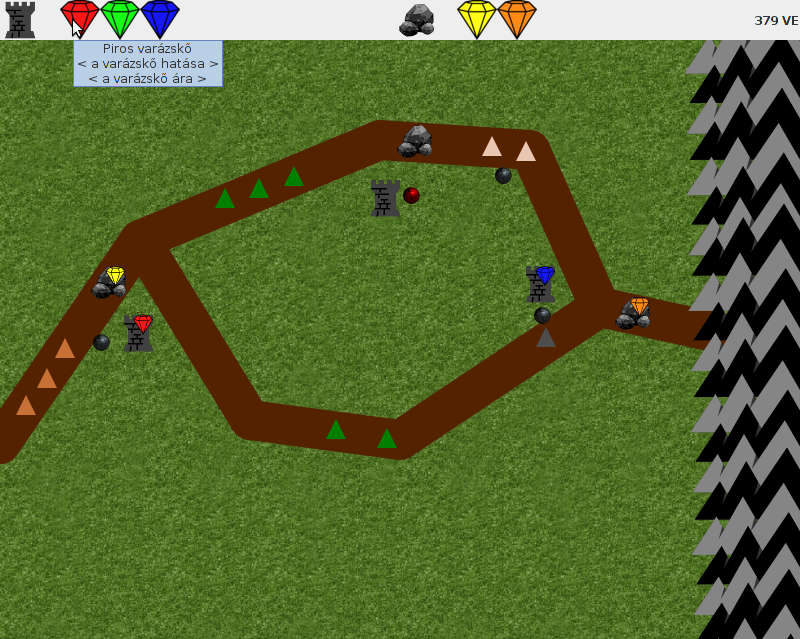
\includegraphics[width=14cm]{images/ch11/screenshot_game.png}
\caption{A játék képe}
\label{fig:screenshot_game}
\end{center}
\end{figure}

Az ablak felső részében a menüsáv, alatta pedig a játéktér foglal helyet.

A menüsávban lévő kis ikonok segítségével a következő funkciók érhetők el (balról jobbra haladva):

\begin{itemize}
\item Torony ikon: Először erre, majd a játéktéren egy megfelelő helyre (nem útra) kattintva egy torony építhető
\item Piros, zöld és kék varázskő ikonok: Először ezekre, majd a játéktéren egy toronyra kattintva egy torony erősíthető a kiválasztott varázskővel
\item Akadály ikon: Először erre, majd a játéktéren egy megfelelő helyre (útra) kattintva egy akadály építhető
\item Sárga és narancssárga varázskő ikonok: Először ezekre, majd a játéktéren egy akadályra kattintva egy akadály erősíthető a kiválasztott varázskővel
\end{itemize}

A menüsáv jobb szélén pedig a jelenleg rendelkezésre álló varázserőnket olvashatjuk le.\\
\\
Ahogyan a fenti ábrán is látszik, az egérmutatót a varázskő ikonokon tartva egy felugró eszköztipp ablakban megjelenik néhány sor szöveg, amely leírja a kiválasztott varázskő nevét, tulajdonságait, és varázserőben mért árát.\\
\\
A játéktér jeleníti meg a csata pillanatnyi állapotát. A barna vonalak az ellenség útvonalai, amelyeken az ablak jobb szélen látható Végzet Hegye felé tartanak.\\
\\
Az egyes ellenségeket különbözű színű háromszögek szimbolizálják. A sötétebb narancssárga embert, a halványrózsaszín hobbitot, a zöld tündét, a szürke pedig törpöt jelent.\\
\\
A tornyok magától értetődő ábrával jelennek meg, az akadályok az utakon pedig egy három szikladarabot ábrázoló kép formájában.\\
\\
Azon tornyok és akadályok képe fölött, amelyek már meg lettek erősítve varázskővel, a rajtuk lévő kő ikonja megjelenik a jobb felső sarokban.\\
\\
A tornyok által az ellenségekre kilőtt lövedékek a fekete, míg a különleges, kettévágó lövedékek a piros golyók.\\
\\
Az alkalmanként leszálló köd az egész játékteret beborító halvány, szürkés átfedés formájában fog megjelenni.\\
\\
Összefoglaló áttekintés a játéktér ikonjairól (nem méretarányosan):

\begin{figure}[ht]
\centering

\subfigure[Torony]{

\includegraphics[width=2cm]{images/ch11/icons/tower.png}
    \label{overview:tower}
}
\subfigure[Akadály]{
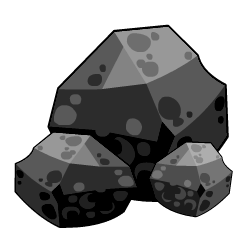
\includegraphics[width=2cm]{images/ch11/icons/obstacle.png}
    \label{overview:obstacle}
}
\subfigure[Varázskő]{

\includegraphics[width=2cm]{images/ch11/icons/blue_gem.png}
    \label{overview:gem}
}
\subfigure[Ellenség]{

\includegraphics[width=2cm]{images/ch11/icons/human.png}
    \label{overview:enemy}
}
\subfigure[Lövedék]{

\includegraphics[width=2cm]{images/ch11/icons/projectile.png}
    \label{overview:projectile}
}
\subfigure[Kettévágó lövedék]{

\includegraphics[width=2cm]{images/ch11/icons/splitter_projectile.png}
    \label{overview:splitter_projectile}
}
\caption{Áttekintés az ikonokról}
\label{fig:icon_overview}
\end{figure}

\newpage

\section{A grafikus rendszer architektúrája}
%\comment{A felület működésének elve, a grafikus rendszer architektúrája (struktúra diagramok). A struktúra diagramokon a prototípus azon és csak azon osztályainak is szerepelnie kell, amelyekhez a grafikus felületet létrehozó osztályok kapcsolódnak.}

\subsection{A felület működési elve}
A grafikus felületet MVC architektúrának megfelelően próbáltuk megtervezni. Minden képernyőn megjelenő objektumnak van egy grafikus párja, ami megvalósítja a \textbf{Drawable} interfészt. A \textbf{View} osztály ilyen objektumokat tárol, és minden kirajzolásnál meghívja ezen objektumok draw metódusát. \\
A megjelenítés push alapú. Ha a modelben történt valami változás (amit hívhatunk egy eseménynek), akkor értesíti a \textbf{View}-t, hogy valami esemény történt, úgy hogy meghívja az eseménynek megfelelő metódust. Kirajzolásnál minden grafikus objektum, lekérdezi a \textbf{Game}-ben lévő párjától az adatait, majd ez alapján kirajzolja magát. Esemény esetén nem történik kirajzolás. Kirajzolás csakis a drawAll() metódus hívásra történik, amit a Game adott időközönként meghív.\\
Az MVC megvalósítás alól kivételt képez a program indulása, amikor is egy egyszerű menü jelenik, amin el lehet indítani a játékot, ezt a \textbf{Menu} osztály végzi. Ez az osztály annyira egyszerű, hogy felesleges ebben is egy MVC-t megvalósítani.\\
A \textbf{Controller} osztály a program elején, a \textbf{Game} és \textbf{View} objektumok létrehozása után feliratkozik a neki megfelelő eseményekre. Ez után már fogadja is az eseményeket.\\
Tervezés során ügyletünk arra is, hogy könnyen bővíthető, cserélhető legyen a rendszer. A \textbf{View} és \textbf{Graphic} osztályokból való származtatással új GUI-t lehet készíteni, anélkül, hogy meglévő kódban kelljen (sokat) változtatni.

\subsection{A felület osztály-struktúrája}
%\comment{Osztálydiagram. Minden új osztály, és azon régiek, akik az újakhoz közvetlenül kapcsolódnak.}

\begin{figure}[H]
\begin{center}
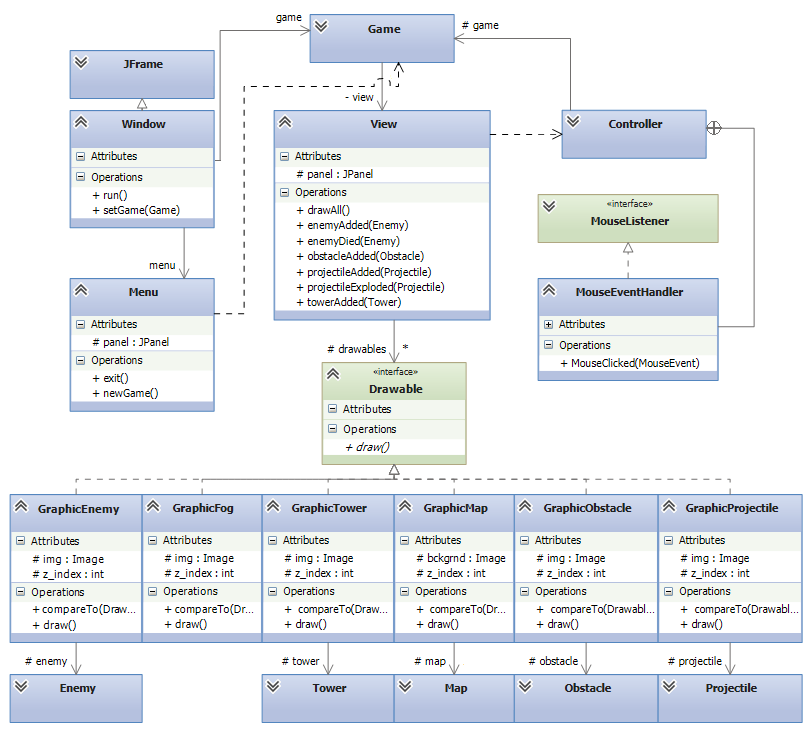
\includegraphics[width=18cm]{images/ch11/very_final_uml_doge_diagram.png}
\caption{Grafikus felület osztálydigaramja}
\label{fig:Graphic_class_diag}
\end{center}
\end{figure}

\pagebreak
\section{A grafikus objektumok felsorolása}
%\comment{Az új osztályok felsorolása. Az régi osztályok közül azoknak a felsorolása, ahol változás volt. Ezek esetén csak a változásokat kell leírni.}

\subsection{Controller}
\begin{itemize}
\item Felelősség \newline
A játék futása közben a felhasználótól érkező eseményeket kezeli, és értesíti róluk a Game-et. Az egyes események kezelését továbbadja a benne lévő eseménykezelő osztályoknak.
\item Attribútumok
	\begin{itemize}
		\item - game: Game: A kontrollerhez tartozó Game onjektum.
	\end{itemize}
\end{itemize}

\subsection{Drawable}
\begin{itemize}
\item Felelősség \newline
Közös alapot biztosít a játékban az összes kirajzolható objektumnak.
\item Interfészek
\begin{itemize}
	\item Comparable<Drawable>: A kirajzolási sorrend megállapítása miatt van erre szükség.
\end{itemize}
\item Attribútumok
	\begin{itemize}
		\item \# img: Image: A kirajzolandó objektum képe.
		\item \# z\_index: int: A kirajzolandó objektum mélységi elhelyezkedése.
	\end{itemize}
\item Metódusok
	\begin{itemize}
		\item + \textit{draw(Graphics)}: Kirajzolja az objektumot.
		\item + compareTo(Drawable): int: Z-index szerint hasonlít össze két Drawable-t.
		\item + \underline{drawRangeCircle}(Graphics2D, Color, int x, int y, int radius): Egy kört rajzol ki az adott koordináták köré, a tornyok és akadályok hatótávolságának jelzésére van.
	\end{itemize}
\end{itemize}

\subsection{Game}
\begin{itemize}
\item Attribútumok
	\begin{itemize}
		\item - view: View: Egy referencia a grafikus megjelenítést végző osztályra.
	\end{itemize}
\end{itemize}

\subsection{GraphicEnemy}
\begin{itemize}
\item Felelősség \newline
Egy ellenség kirajzolása.
\item Ősosztályok\newline
Drawable
\item Attribútumok
	\begin{itemize}
		\item \# enemy: Enemy: A kirajzolandó ellenség.
	\end{itemize}
\item Metódusok
	\begin{itemize}
		\item + draw(Graphics): Kirajzolja az ellenséget.
		\item + equals(Object): boolean: Megadja, hogy két Graphic objektum egyenlő-e (ugyanazt a játékbeli objektumot reprezentálja).
	\end{itemize}
\end{itemize}

\subsection{GraphicFog}
\begin{itemize}
\item Felelősség \newline
A köd kirajzolása.
\item Ősosztályok\newline
Drawable
\item Metódusok
	\begin{itemize}
		\item + draw(Graphics): Kirajzolja a ködöt.
	\end{itemize}
\end{itemize}

\subsection{GraphicGem}
\begin{itemize}
\item Felelősség \newline
Egy varázskő kirajzolása lerakás közben.
\item Ősosztályok \newline
Drawable
\item Attribútumok
	\begin{itemize}
		\item \# pos: Vector: A varázskő jelenlegi helye.
	\end{itemize}
\item Metódusok
	\begin{itemize}
		\item + draw(Graphics): Kirajzolja a varázskövet.
		\item + getPosition(): Vector: Visszaadja a varázskő helyét.
	\end{itemize}
\end{itemize}

\subsection{GraphicMap}
\begin{itemize}
\item Felelősség \newline
A pálya kirajzolása.
\item Ősosztályok\newline
Drawable
\item Attribútumok
	\begin{itemize}
		\item \# map: Map: A kirajzolandó pálya.
		\item \# mountains: Image: A pálya jobb oldalán lévő hegyek képe.
	\end{itemize}
\item Metódusok
	\begin{itemize}
		\item + draw(Graphics): Kirajzolja a pályát.
		\item + equals(Object): boolean: Megadja, hogy két Graphic objektum egyenlő-e (ugyanazt a játékbeli objektumot reprezentálja).
	\end{itemize}
\end{itemize}

\subsection{GraphicObstacle}
\begin{itemize}
\item Felelősség \newline
Egy akadály kirajzolása.
\item Ősosztályok \newline
Drawable
\item Attribútumok
	\begin{itemize}
		\item \# obstacle: Obstacle: A kirajzolandó akadály.
		\item \# gemImage: Image: Az akadályra rakott varázskő képe.
	\end{itemize}
\item Metódusok
	\begin{itemize}
		\item + draw(Graphics): Kirajzolja az akadályt.
		\item + equals(Object): boolean: Megadja, hogy két Graphic objektum egyenlő-e (ugyanazt a játékbeli objektumot reprezentálja).
		\item + setGem(): Frissíti a kirajzolandó varázskő képét.
	\end{itemize}
\end{itemize}

\subsection{GraphicProjectile}
\begin{itemize}
\item Felelősség \newline
Egy lövedék kirajzolása.
\item Ősosztályok\newline
Drawable
\item Attribútumok
	\begin{itemize}
		\item \# projectile: Projectile: A kirajzolandó lövedék.
	\end{itemize}
\item Metódusok
	\begin{itemize}
		\item + draw(Graphics): Kirajzolja a lövedéket.
		\item + equals(Object): boolean: Megadja, hogy két Graphic objektum egyenlő-e (ugyanazt a játékbeli objektumot reprezentálja).
	\end{itemize}
\end{itemize}

\subsection{GraphicTower}
\begin{itemize}
\item Felelősség \newline
Egy torony kirajzolása.
\item Ősosztályok\newline
Drawable
\item Attribútumok
	\begin{itemize}
		\item \# tower: Tower: A kirajzolandó torony.
		\item \# gemImage: Image: A toronyra rakott varázskő képe.
	\end{itemize}
\item Metódusok
	\begin{itemize}
		\item + draw(Graphics): Kirajzolja a tornyot.
		\item + equals(Object): boolean: Megadja, hogy két Graphic objektum egyenlő-e (ugyanazt a játékbeli objektumot reprezentálja).
		\item + setGem(): Frissíti a kirajzolandó varázskő képét.
	\end{itemize}
\end{itemize}


\subsection{Menu}
\begin{itemize}
\item Felelősség \newline
A játék főmenüjét valósítja meg, amivel új játékot lehet indítani, ezen belül kiválasztani a pályát és a missziót.
\item Attribútumok
	\begin{itemize}
		\item \# panel: JPanel: A menü kirajzolásához használt JPanel.
	\end{itemize}
\item Metódusok
	\begin{itemize}
		\item + exit(): Bezárja a játék ablakait, és kilép a programból.
		\item + newGame(): Új játék indítását kezdeményezi.
		\item + run(): Elindítja a menü futását.
	\end{itemize}
\end{itemize}

\subsection{MouseEventHandler}
\begin{itemize}
\item Felelősség  \newline
Az egérkattintás eseményeket kezeli le.
\item Interfészek
\begin{itemize}
	\item MouseListener
\end{itemize}
\item Metódusok
	\begin{itemize}
		\item + MouseClicked(MouseEvent): Egérkattintáskor hívódik meg, kezeli az eseményt. Az egérkattintás pozíciójától függően meghívja a megfelelő metódust a Game-ben.
	\end{itemize}
\end{itemize}

\subsection{View}
\begin{itemize}
\item Felelősség \newline
A játék kirajzolása, azaz a Game osztály állapotának megjelenítésa a képernyőn.
\item Attribútumok
	\begin{itemize}
		\item - panel: JPanel: A játék kirajzolásához használt JPanel
		\item - drawables: List<Drawable>: A játékban kirajzolandó dolgok (ellenségek, tornyok, stb.) listája rendezve, hogy jó sorrenben legyen az objektumok kirajzolva.
		\item - mapPanel: JPanel: A játéknak a játékterét (pálya, ellenségek, tornyok, stb.) megjelenítő JPanel.
		\item - magicPanel: JPanel: A játék ezköztárát megjelenítő JPanel.
		\item - placing: Drawable: Azt az objektumot tárolja, ami épp lerakás alatt van, így ekkor is meg lehet jeleníteni.
	\end{itemize}
\item Metódusok
	\begin{itemize}
		\item + addDrawable(Drawable): Berak egy Drawable-t a kirajzolandó objektumok listájába.
		\item + drawAll(): Kirajzolja a játék jelenlegi állását.
		\item + enemyAdded(Enemy): A Game hívja meg amikor új ellenség kerül a pályára, frissíti a View adatstruktúráit.
		\item + enemyDied(Enemy): A Game hívja meg amikor meghal egy ellenség, frissíti a View adatstruktúráit.
		\item + gameLost(): Kirajzolja a vesztes játék végi üzenetet.
		\item + gameWon(): Kirajzolja a nyertes játék végi üzenetet.
		\item + getPanel(): Visszaadja a ``panel'' tagváltozót.
		\item + magicChange(int): Megváltoztatja a kiírt varázserő értéket a paraméterként kapottra.
		\item + obstacleAdded(Obstacle): A Game hívja meg amikor új akadály kerül a pályára, frissíti a View adatstruktúráit.
		\item + obstacleEnchanted(Obstacle): Frissíti egy meglévő akadály aktív varázskövét.
		\item - setButtonLook(JButton, ImageIcon): Beállítja egy JButton kinézetét.
		\item + setPlacing(Drawable): Beállítja az éppen lerakás alatt álló objektumot.
		\item + towerAdded(Tower): A Game hívja meg amikor új torony kerül a pályára, frissíti a View adatstruktúráit.
		\item + towerEnchanted(Tower): Frissíti egy meglévő torony aktív varázskövét.
		\item + projectileAdded(Projectile): A Game hívja meg amikor új lövedék kerül a pályára, frissíti a View adatstruktúráit.
		\item + projectileExploded(Projectile): A Game hívja meg amikor egy lövedék megsemmisül, frissíti a View adatstruktúráit.
		\item - winLoseScreen(String, Image): Kirajzolja a játék végi üzenetet és képet (nyerés/vesztés).
	\end{itemize}
\end{itemize}

\subsection{Window}
\begin{itemize}
\item Felelősség \newline
A játék fő ablaka, ez jeleníti meg a menüt és aztán magát a játékot.
\item Ősosztályok\newline
JFrame
\item Attribútumok
	\begin{itemize}
		\item - menu: Menu: A játék menü objektumát tárolja.
		\item - game: Game: A játék Game objektumát tárolja.
	\end{itemize}
\item Metódusok
	\begin{itemize}
		\item + setGame(Game): Beállítja azt a Game objektumot, amit a kezelőfelület meg fog jeleníteni. A menü fogja meghívni a pálya- és misszióválasztás után.
	\end{itemize}
\end{itemize}

\section{Kapcsolat az alkalmazói rendszerrel}
%\comment{Szekvencia-diagramokon ábrázolni kell a grafikus rendszer működését. Konzisztens kell legyen az előző alfejezetekkel. Minden %metódus, ami ott szerepel, fel kell tűnjön valamelyik szekvenciában. Minden metódusnak, ami szekvenciában szerepel, szereplnie kell a %valamelyik osztálydiagramon.}

\begin{figure}[H]
\begin{center}
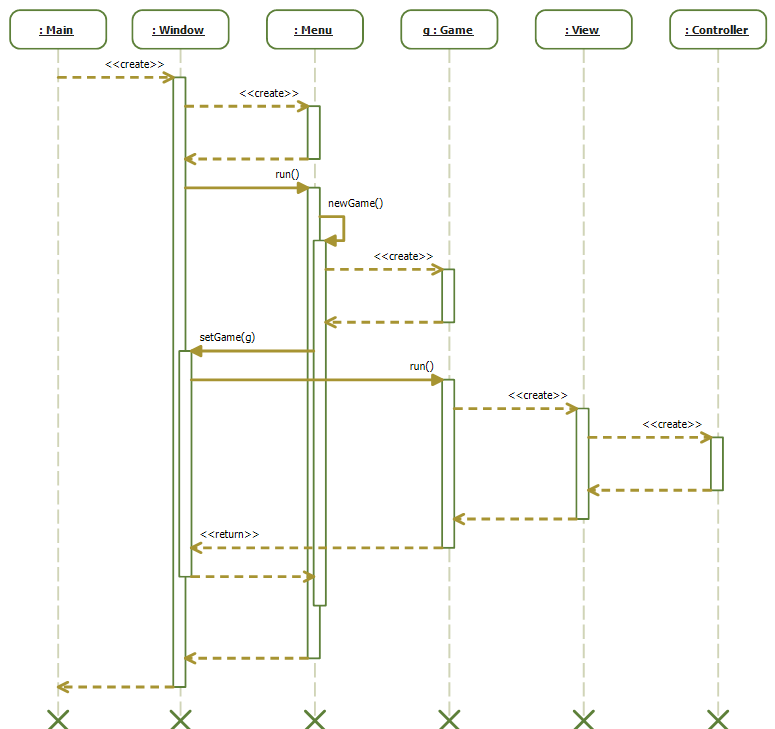
\includegraphics[width=18cm]{images/grafikaSeq/init.png}
\caption{Játék inicializálása.}
\label{fig:Graphic_initialize}
\end{center}
\end{figure}

\begin{figure}[H]
\begin{center}
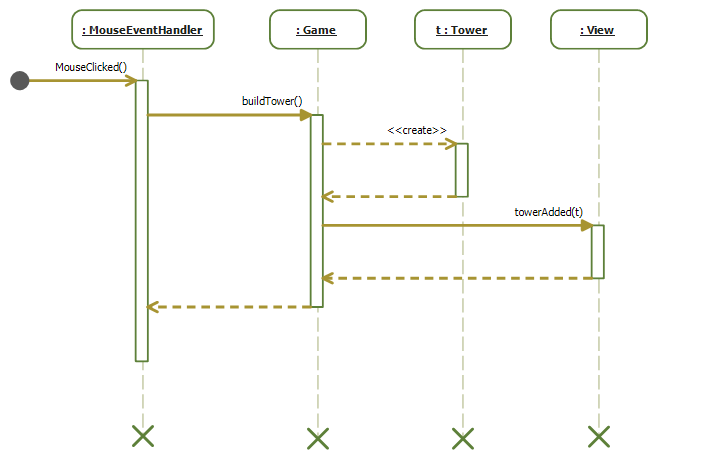
\includegraphics[width=18cm]{images/grafikaSeq/mouseTower.png}
\caption{Egérkattintásra torony lerakása.}
\label{fig:Graphic_mouse_tower}
\end{center}
\end{figure}

\begin{figure}[H]
\begin{center}
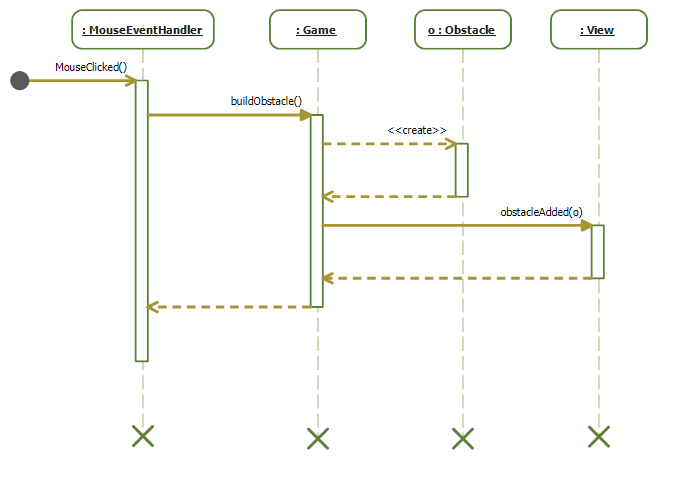
\includegraphics[width=18cm]{images/grafikaSeq/mouseOb.png}
\caption{Egérkattintásra akadály lerakása.}
\label{fig:Graphic_mouse_obstacle}
\end{center}
\end{figure}

\begin{figure}[H]
\begin{center}
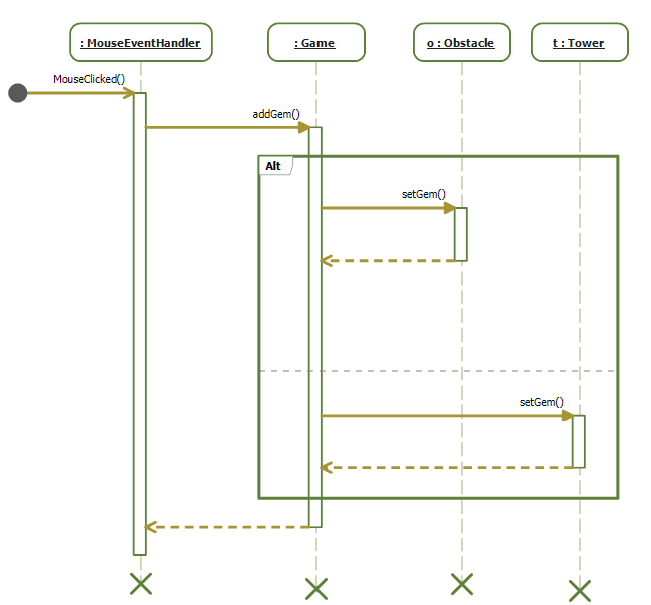
\includegraphics[width=18cm]{images/grafikaSeq/mouseEnch.png}
\caption{Egérkattintásra torony vagy akadály varázskővel felruházása.}
\label{fig:Graphic_mouse_enchant}
\end{center}
\end{figure}

\begin{figure}[H]
\begin{center}
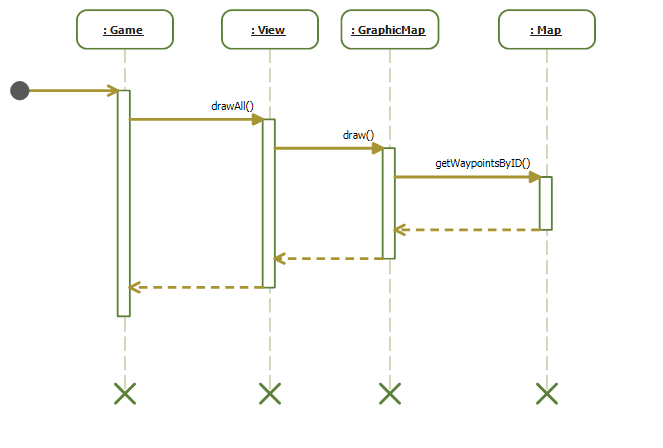
\includegraphics[width=18cm]{images/grafikaSeq/step1.png}
\caption{Az egész játék kirajzolása.(Map része)}
\label{fig:Graphic_drawAll_Map}
\end{center}
\end{figure}

\begin{figure}[H]
\begin{center}
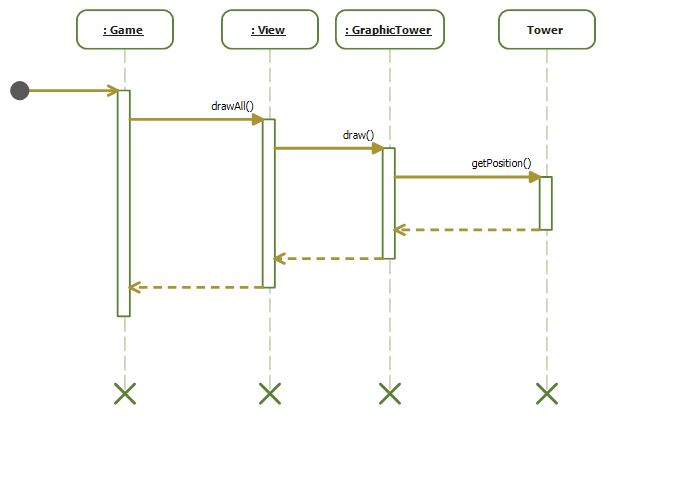
\includegraphics[width=18cm]{images/grafikaSeq/step2.png}
\caption{Az egész játék kirajzolása.(Tower része)}
\label{fig:Graphic_drawAll_Tower}
\end{center}
\end{figure}

\begin{figure}[H]
\begin{center}
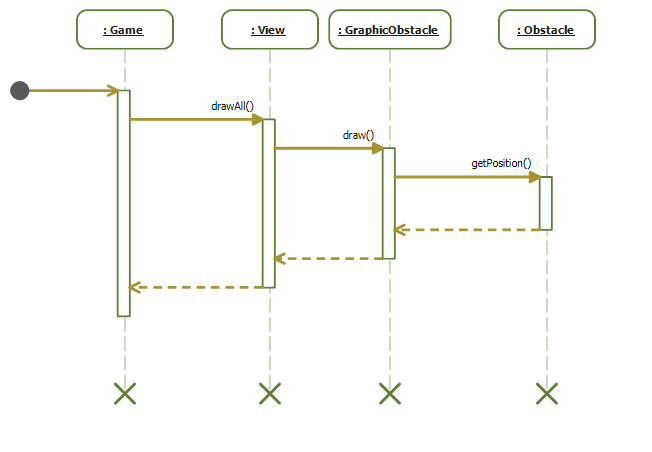
\includegraphics[width=18cm]{images/grafikaSeq/step3.png}
\caption{Az egész játék kirajzolása.(Obstacle része)}
\label{fig:Graphic_drawAll_Obstacle}
\end{center}
\end{figure}

\begin{figure}[H]
\begin{center}
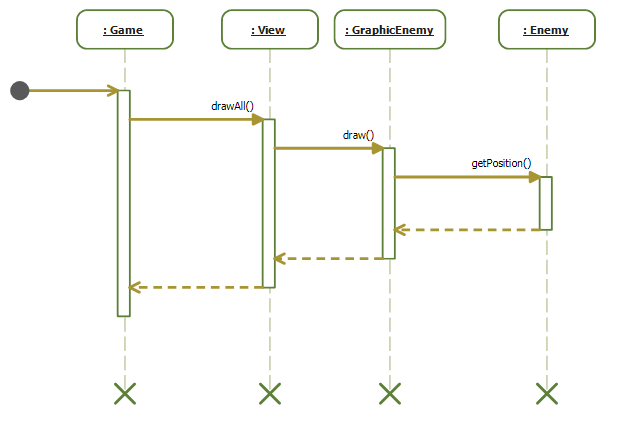
\includegraphics[width=18cm]{images/grafikaSeq/step4.png}
\caption{Az egész játék kirajzolása.(Enemy része)}
\label{fig:Graphic_drawAll_Enemy}
\end{center}
\end{figure}

\begin{figure}[H]
\begin{center}
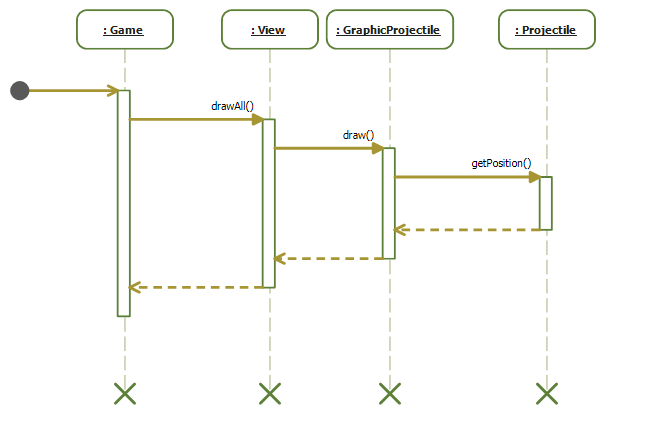
\includegraphics[width=18cm]{images/grafikaSeq/step5.png}
\caption{Az egész játék kirajzolása.(Projectile része)}
\label{fig:Graphic_drawAll_Projectile}
\end{center}
\end{figure}

\begin{figure}[H]
\begin{center}
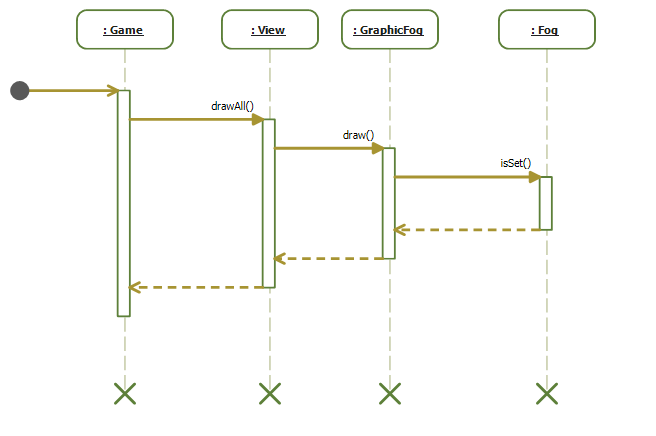
\includegraphics[width=18cm]{images/grafikaSeq/step6.png}
\caption{Az egész játék kirajzolása.(Fog része)}
\label{fig:Graphic_drawAll_Fog}
\end{center}
\end{figure}

\begin{figure}[H]
\begin{center}
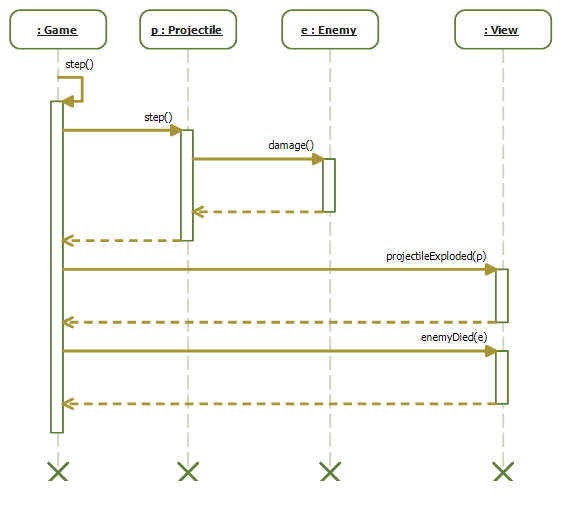
\includegraphics[width=18cm]{images/grafikaSeq/proj_Enemy_del.png}
\caption{Ellenség és lövedék törlése.}
\label{fig:Graphic_enemy/projectile_del}
\end{center}
\end{figure}